% !TEX root = ../../Main.tex
\section{Out-of-Sample Behaviour: The Held-Out Year}
\label{Section:OutOfSample}

The split of \Cref{Equation:Split} trains on 2015 to 2023, selects among episodes on 2024, and does not use 2025 at all. Because the trained weights are stored, 2025 can be scored on its own.

\textbf{The result is negative.} \Cref{Tables:TestYear} gives the figures. Five of the seven pairs lose money in 2025. The mean model return is $-6.8\%$, while the mean market move would have made money. Only USD/CHF, at $+5.0\%$, and USD/JPY, at $+0.6\%$, are positive.

% !TEX root = ../Main.tex
\begin{table}[htb!]
\centering
\footnotesize
\caption{The held-out year against the validation year and the full window. 2025 was seen by no part of the training or selection procedure; 2024 was used to choose which episode's weights were kept. The last column is the move of the pair itself in 2025.}
\label{Tables:TestYear}
\begin{tabular}{@{}lrrrr@{}}
\toprule
\textbf{Pair} & \textbf{2025 (Test)} & \textbf{2024 (Validation)} & \textbf{Full Window} & \textbf{2025 Market} \\
\midrule
AUD/USD & $-11.7\%$ & $+72.4\%$ & $+102.5\%$ & $+7.6\%$ \\
EUR/USD & $-1.2\%$ & $-5.9\%$ & $+73.9\%$ & $+13.5\%$ \\
GBP/USD & $-22.9\%$ & $-3.6\%$ & $+124.1\%$ & $+7.6\%$ \\
NZD/USD & $-5.0\%$ & $+11.0\%$ & $+56.4\%$ & $+2.8\%$ \\
USD/CAD & $-13.4\%$ & $+28.8\%$ & $+226.6\%$ & $-4.6\%$ \\
USD/CHF & $\mathbf{+5.0\%}$ & $+3.7\%$ & $+50.6\%$ & $-12.8\%$ \\
USD/JPY & $+0.6\%$ & $+7.6\%$ & $+15.7\%$ & $-0.7\%$ \\
\midrule
\textbf{Portfolio} & $\mathbf{-9.8\%}$ & --- & $+91.3\%$ & --- \\
\bottomrule
\end{tabular}
\end{table}

The comparison with 2024 is the important part, and \Cref{Figure:YearlyExcess} shows it directly. 2024 is the best year in the whole sample, with a mean excess return of $+16.4$ percentage points over the benchmark. 2025 is the worst, at $-8.7$. The difference between the two years is that 2024 was used to decide which episode's weights were kept, and 2025 was not used for anything. This gap is the measured effect of selection. It is the reason the full-window figures in \Cref{Tables:PairResults} are called an in-sample result throughout this thesis.

\begin{figure}[htb!]
\centering
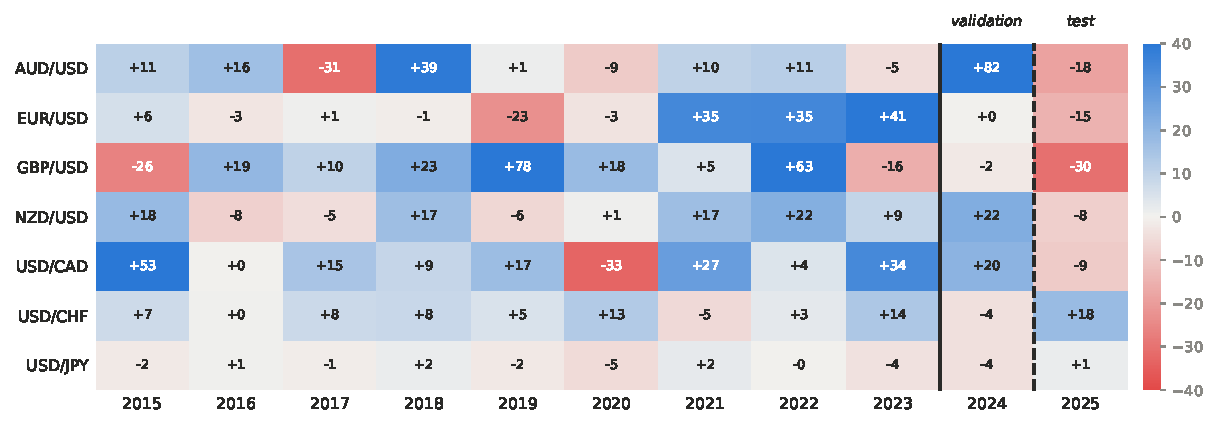
\includegraphics[width=\textwidth]{Images/YearlyExcess.pdf}
\caption{Yearly return of each agent minus the return of buying and holding the same pair, in percentage points. Blue marks outperformance of the benchmark. The solid line marks the end of the training data and the dashed line the end of the validation year, so only the last column was not seen by any part of the procedure.}
\label{Figure:YearlyExcess}
\end{figure}

There is a market explanation for the direction of the 2025 result. It is worth giving because it leads to a useful conclusion. In 2025 there was a broad dollar reversal. EUR/USD rose $13.5\%$, its largest yearly move in the eleven years, and the dollar became weaker against five of the seven pairs. The agents were trained on a decade in which the dollar mostly became stronger, and six of the seven were positioned for that. The seventh, USD/CHF, is the least directional model of the seven. It holds the fewest positions and has the lowest beta, and it is the one that made money. This agrees with the rest of the evidence and is not a coincidence. The model that depends least on the direction of the market is the one that held up when that direction changed.

The individual results should be read, and not only their average, because the models do not fail in the same way. GBP/USD is the worst, at $-22.9\%$. It is the most aggressive model of the seven. It trades near full size and has the deepest drawdown over the full window, so a year that goes against it costs a lot. USD/CAD loses $13.4\%$ and AUD/USD $11.7\%$. Both are leveraged-exposure models of \Cref{Section:AlphaBeta}, so a reversal in the direction of their beta is exactly the event that hurts them. EUR/USD loses only $1.2\%$, although the pair moved $13.5\%$. This agrees with its beta near zero: it did not take part in the reversal in either direction.

The two models that held up are the two that held the least. USD/CHF returned $+5.0\%$ while its pair fell $12.8\%$. That is an excess return of $17.8$ percentage points, and its best year against the benchmark in the whole sample. USD/JPY returned $+0.6\%$. This is not skill. It only means that the model was not exposed to the pairs that moved. Together, the two show the pattern: the models that depended least on the direction of the market were the ones that held up when that direction changed.

One year is a small sample, and no conclusion should be drawn from it beyond the obvious one. The held-out year limits what can be claimed, but it is not a final judgement on the design. The design kept trading in a sensible way on data it had never seen. It lost money doing so, in a year whose direction was not in its training data.